\documentclass[a4paper]{llncs}

\usepackage[centertags]{amsmath}
\usepackage{amsfonts,graphicx,subcaption}
\newcounter{enumroman}
\newcommand{\var}{\mathop{\rm Var}}
\newcommand{\cov}{\mathop{\rm cov}}
\newenvironment{romanitems}{\begin{list}{\bfseries(\roman{enumroman})\hfill}{\usecounter{enumroman}\setlength{\labelwidth}{\leftmargin}\addtolength{\labelwidth}{-1\labelsep}\topsep=0mm plus 2pt\itemsep=0mm plus 1pt\parsep=0mm\itemsep=0mm plus 1pt\itemindent=0mm}}{\end{list}}

\title{Multi-instance Learning as an Adaptive Approach to Multiset Clustering}
\author{Marek D\v{e}di\v{c}\inst{1,2}, Luk\'a\v{s} Bajer\inst{2}, Martin Hole\v{n}a\inst{3}}
\institute{Faculty of Nuclear Sciences and Physical Engineering, Czech Technical University, Trojanova 13, Prague, Czech Republic \and Cisco Systems, Inc., Karlovo n\'am\v{e}st\'{\i} 10, Prague, Czech Republic \and Institute of Computer Science, Czech Academy of Sciences, Pod vod\'arenskou v\v{e}\v{z}\'{\i}~2, Prague, Czech Republic}

\begin{document}
\bibliographystyle{splncs04}

\maketitle

\section{Introduction}

Multi-instance learning (MIL) belongs to recently fast developing areas of machine learning. Though it is a supervised learning method, we use it here for unsupervised learning -- clustering.  Whereas traditional clustering clusters points, multi-instance clustering clusters multisets of points, also called bags. A key prerequisite for such an application of multi-instance learning is that loss functions for clustering, originally proposed for points, are adapted for bags. Here, the adaptation of three sophisticated loss functions is outlined: contrastive predictive coding, triplet loss and magnet loss. Their adaptation is currently being validated on 21 datasets. First results of that validation are exemplified at the end of this extended abstract.

\section{Multi-instance Learning and Clustering}

The MIL paradigm is a type of representation learning for data with some internal structure. Therefore, it views a sample as a bag of an arbitrary number of objects. Basic MIL ingredients are samples from a space $ \mathcal{X} $ and their corresponding labels from a space $\mathcal{Y} $. Compared to usual supervised learning, MIL replaces individual instances with bags of instances from the space $ \mathcal{X} $ such that every instance in $ \mathcal{X} $ belongs to at least one bag.

The notion of an instance-level label is dropped in this interpretation, the bag is an atomic unit of interest. Labels are only defined on the level of bags. In order for these bag labels to be learned, an embedding function of the form $\phi:\mathcal{B}\to\bar{\mathcal{X}}$ must be defined, where $\mathcal{B}$ is the set of considered bags, and $\bar{\mathcal{X}}$ is a latent space. Using  $\phi$, each bag can be represented by an object $\phi (B)\in\bar{\mathcal{X}}$, which makes it possible to use any off-the-shelf supervised learning algorithm acting on $\bar{\mathcal{X}}$. Among the simplest embedding functions are, e.g. the element-wise minimum, maximum and mean. A more complicated embedding function may be, for example, computed by a neural network.

Clustering is a prime example of a problem typically associated with unsupervised learning. While \cite{wang_solving_2000} presents a clustering of bags using a modified Hausdorff distance on bags and \cite{kohout_network_2018} presents a clustering using maximum mean discrepancy, we have chosen a different approach based on the embedded-space paradigm for MIL. The embedding can be actually written $\phi = \phi( B, \mathbf{\theta})$, where $B$ is from some considered set $\mathcal{B}$ of bags and $\theta$ are the parameters of the embedding, typically learned during training.	A clustering-loss function $L_C$ is chosen on the subsets of the latent space. Given such clustering-loss function, the actual loss for the embedding $\phi$ and its parameters $\theta$ can be computed as
\begin{gather}
	L \left( \phi, \mathbf{\theta} \right) = L_C \left( \left\{ \phi \left( B, \mathbf{\theta} \right) \middle| B \in \mathcal{B} \right\} \right)
\end{gather}
If the clustering-loss	$L_C$ is chosen correctly, minimizing  $L$ over the learning period will yield a latent space $\bar{\mathcal{X}}$ in which the bags are already naturally clustered according to the design of the clustering-loss function. Applying any off-the shelf clustering algorithm on  $\bar{\mathcal{X}}$ will then give good results. How to choose the clustering-loss function $L_C$ is the focus of Section 3.

\section{Adaptation of Loss Functions for Multiset Clustering}

In this section, three ways of constructing the above mentioned clustering-loss function $L_C$ are explored.

\emph{Contrastive predictive coding} (CPC) is a technique first introduced by \cite{oord_representation_2019}. It represents time series by modelling future data from the past. The core concept taken from CPC is a loss function called InfoNCE in the prior art. Given a set $\mathbb{X} = \{x_1,\dots,x_N\}$ containing samples from $p (x_{t=k}|c_t)$ where $c_t$ is a context provided by an autoregressive model $f_k$ summarizing latent representations up to the time point $t$, the InfoNCE loss is defined:
\begin{gather}
	L_\text{NCE} = - \underset{\mathbb{X}}{\mathbb{E}} \left[\log f_k \left( x_{t + k}, c_t \right) - \log \sum_{x_j \in \mathbb{X}} f_k \left( x_j, c_t \right) \right]
\end{gather}

The actual application to MIL is based on the following idea. If a bag is split into two parts, it is reasonable to expect that the representations of these two parts would be close to one another. On the other hand the representations of two mismatched bags $B^{ (1) }_{k_1}$ and $B^{ (1) }_{k_2}$ should be far apart. A matrix $\mathbf{D}\in\mathbb{R}^{n\times n}$ is defined
\begin{gather}\label{adc}
	\mathbf{D}_{ij} = \| \phi \left( B_i^{(1)} \right) - \phi \left( B_j^{(2)} \right) \|^2.
\end{gather}
Then the final loss for the CPC method is
\begin{gather}
	L_\mathrm{CPC} = \frac{1}{n} \sum_{i = 1}^n \left( \log \left( \mathbf{D}_{ii} \right) - \log \sum_{\substack{j = 1 \\ j \neq i}}^n \mathbf{D}_{ij} \right).
\end{gather}

Let $\{( \mathbf{x}_i, y_i ) \}_{i = 1}^n$ be a training dataset with $x_i\in \mathbb{R}^d$ and $y_i$ discrete class labels. In the definition of the next loss function, called \emph{triplet loss}, a helper matrix $\mathbf{y}\in\{0,1\}^{n\times n}$ is used such that $\mathbf{y}_{ij} =1$ iff $y_i = y_j$, and another matrix $\eta\in\{0,1\}^{n\times n}$ indicates target neighbours: $\eta_{ij} = 1$ iff $x_j$ is a target neighbour of $x_i$. This loss function reflects the idea that an input should be close to its target neighbours, whereas inputs of different classes should be far from one another. To adapt the original method to bags, the matrix $\mathbf{y}$ is defined in the same way, only with labels on the level of bags, and $\eta_{ij} = 1$ iff the bag $B_j$ is a target neighbour for the bag $B_i$. Then, using the matrix D defined in (\ref{adc}), the triplet loss function can be expressed as
\begin{gather}
	L_\mathrm{triplet} = \sum_{ij} \eta_{ij} D_{ij} + c \sum_{ijl} \eta_{ij} \left( 1 - y_{il} \right) \max\left(0, D_{il} - D_{ij} \right).
\end{gather}
where  $c > 0$ is a hyper-parameter. Although \cite{weinberger_distance_2006} suggest finding  $\eta$ as the k-nearest neighbours, we simplified $L_\mathrm{triplet}$ by setting $\eta_{ij} = \mathbf{y}_{ij},i,j=1,\dots,n$.

\emph{Magnet loss} is an enhancement of the triplet loss, first introduced by \cite{rippel_metric_2016}. Whereas the triplet loss function essentially goes over all triplets of a data point, its target neighbour and a point from a different class and optimizes their distances, magnet loss maintains an explicit model of the distributions of different classes in the representation space. Differently to the triplet loss, for which the target neighbourhood is set a priori and is based on similarity in the original input space, magnet loss uses similarity in the space of representations and updates it periodically. Let $\{( B_i, y_i) \}_{i = 1}^n$ be a training dataset with inputs $x_i\in \mathbb{R}^d$, $y_i$ be one of $C$ discrete class labels, and $r_i=\phi (B_i)$. For each class $c$, $K$ cluster assignments are obtained with the K-means++ algorithm \cite{macqueen_methods_1967,arthur_k-means++:_2006} where $K\in \mathbb{N} $ is a hyperparameter of the method. Let $\mu^c_k$ be the center of the $k$-th cluster, $\mathbf{\mu} (r_i)$ be the center of the cluster to which the representation of $B_i$ belongs, and $N_i$ be the distance of its representation from the center of the cluster. Denote $\sigma^2 = \frac{1}{n - 1} \sum_{i = 1}^n N_i$. For each $r_i$, the dissimilarity to all the inputs of different classes is calculated as
\begin{gather}
	M_i = \sum_{c \neq y_i} \sum_{k = 1}^K \exp \left( - \frac{1}{2 \sigma^2} N_i^2\right)
\end{gather}
The magnet loss is then defined
\begin{gather}
	L_\text{magnet} = \frac{1}{n} \sum_{i = 1}^n \left( -\exp \left( - \frac{1}{2 \sigma^2} N_i - \alpha \right)+\log M_i \right).
\end{gather}
where  $\alpha \in \mathbb{R} $ is a hyper-parameter of the method.

\section{Ongoing Experimetnal Validation}

At the moment, an extensive experimental validation and comparison of the above multi-instance variants of three clustering loss functions is being performed, on 20 sets of benchmark data and one real-world dataset. The experiments are still in a very early stage, that is why only two examples of first results are given here for illustration. For one of the used datasets, Musk2 \cite{dietterich_solving_1997}, Figure \ref{fig:musk2} shows the evolution of the values of two performance metrics, accuracy of a kNN classifier built on the embedding, and the silhouette coefficient of the resulting clustering, during learning.

\begin{figure}
	\begin{subfigure}[t]{0.49\textwidth}
		\centering
		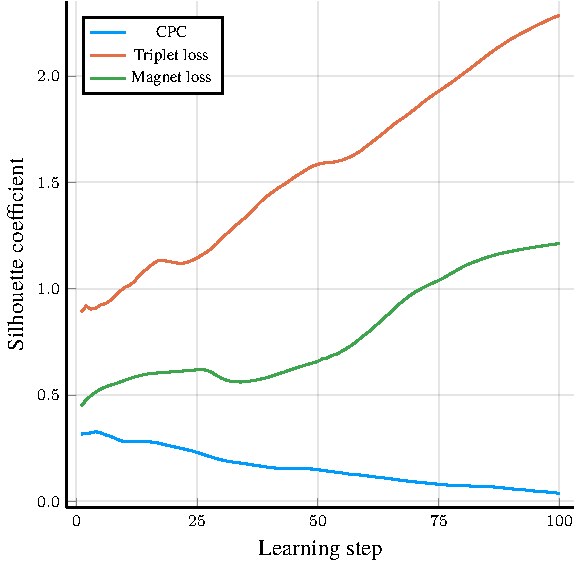
\includegraphics[width=\textwidth]{images/musk2-ratio/musk2-ratio.pdf}
		\caption{The value of the silhouette coefficient}
	\end{subfigure}
	\begin{subfigure}[t]{0.49\textwidth}
		\centering
		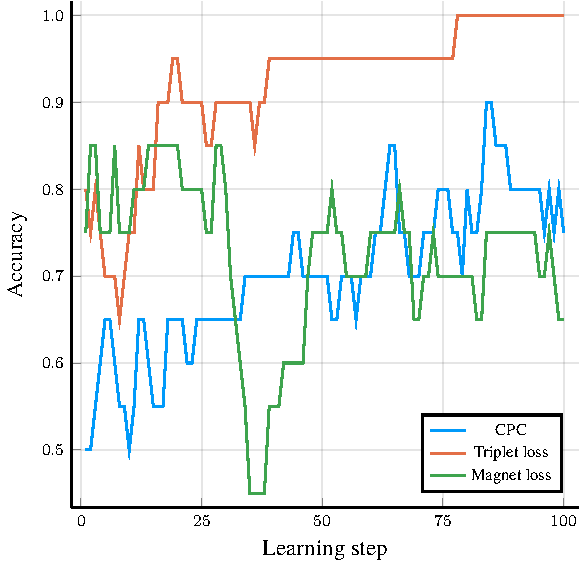
\includegraphics[width=\textwidth]{images/musk2-accuracy/musk2-accuracy.pdf}
		\caption{The accuracy of a kNN classifier built on the embedding}
	\end{subfigure}
	\caption{Performance measures over the learning period on the Musk2 dataset\cite{dietterich_solving_1997}}\label{fig:musk2}
\end{figure}

\section{Conclusion}

This work in progress is a small contribution to the rather new field of multi-instance clustering, an unsupervised counterpart of multi-instance learning.  It consists in the adaptation of three sophisticated clustering loss functions, contrastive predictive coding, triplet loss and magnet loss, to the multi-instance setting. The proposed adaptations are currently undergoing extensive experimental validation and comparison. As the experiments are still in a very early stage, any assessment of their results would be premature. All results and their statistical analysis will be available at the workshop.

\enlargethispage{\baselineskip}
\subsection*{Acknowledgment}

The research reported in this paper has been supported by the Czech Science Foundation (GA\v{C}R) grant 18-18080S.

\bibliography{zotero}

\end{document}
